\section{Introduction}
\label{sec:introduction}

% state the learning objective 
The objective of this laboratory assignment is to study a circuit with four meshes containing a
voltage source $V_a$, a current source $I_d$, and two linearly dependent sources: a voltage controlled current source $I_b$ and a current controlled voltage source $V_c$. The circuit also contains seven Resistors from $R_1$ to $R_7$ as it is shown in Figure~\ref{fig:Circuit_Base}.

In Section~\ref{sec:analysis}, two different theoretical analysis of the circuit are
presented using the mesh method and the nodal method. In Section~\ref{sec:simulation}, the circuit is analysed by
simulation, and the results are compared to the theoretical ones obtained in
Section~\ref{sec:analysis}. The conclusions of this study are outlined in
Section~\ref{sec:conclusion}.

\begin{figure}[h] \centering
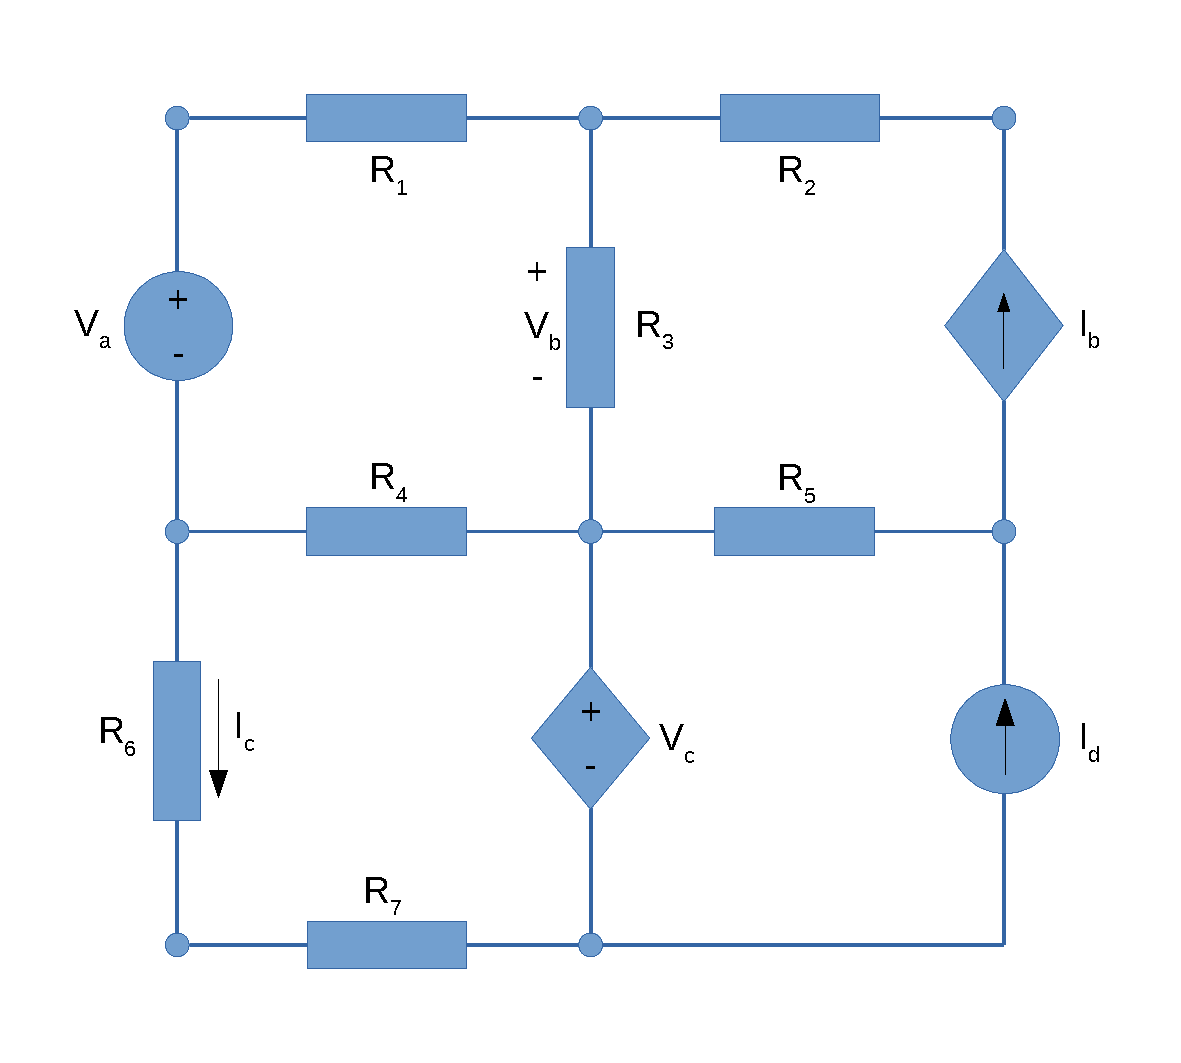
\includegraphics[width=0.5\linewidth]{Circuit.pdf}
\caption{Circuit analysed.}
\label{fig:Circuit_Base}
\end{figure}

